
\chapter{Desenvolvimento dos protótipos}
% Label para referenciar
\label{desenvolvimento-prototipos}

% Diminuir espaçamento entre título e texto
\vspace{-1.9cm}

% Texto do capítulo

  Este capítulo apresenta o cenário proposto para o estudo de caso, bem
  como o desenvolvimento dos protótipos com suas fases de implementação, iniciando
  pela elicitação dos requisitos seguindo a abordagem \ac{REST}.
  
  Como serão desenvolvidos dois protótipos com o objetivo de compara-los um com o outro,
  iniciaremos o desenvolvimento com o \textit{framework} Django e por fim faremos o desenvolvimento
  com o ambiente Node.Js e \textit{framework} Express.Js formando assim a aplicação proposta
  
\section{O escopo do projeto}
\label{escopo-projeto}

  Com base nos aspectos abordados ao longo deste trabalho, 
  esta seção visa apresentar o desenvolvimento de um Web Service seguindo os padrões \ac{REST} e a utilização 
  de um banco de dados relacional Postgres para a persistência dos dados.
  
  Tal serviço possuirá métodos que serão consumidos por dispositivos clientes.

\subsection{Levantamento Requisitos}
\label{levantamento-requisitos}

  Utilizaremos o mesmo exemplo citado por \cite{Pereira:2013} em seu livro. =)
  Devo fazer uma pesquisa aqui?

\subsubsection{Elicitação de requisitos}

  Analisando-se o resultado obtido da aplicação dos métodos de levantamento
  de requisitos utilizados é possível destacar os seguintes requisitos candidatos

  \begin{compactitem}
    \item[a)] A aplicação \ac{API} \ac{REST} deverá ser compatível com todas as versões para computadores com os navegadores 
    web Mozilla Firefox e Google Chrome..
    \item[b)] Não utilizar técnicas de autenticação na API.
    \item[c)] A \ac{API} \ac{REST} deverá responder as requisições do cliente através da representação em JSON.
    \item[d)] A \ac{API} \ac{REST} deverá persistir os dados em Postgres.
    \item[e)] A \ac{API} \ac{REST} deverá ter um recurso chamado Pessoas.
    \item[e)] A \ac{API} \ac{REST} deverá prover estratégias para manipular as ações de CRUD de uma pessoa(s)
    \item[e)] A \ac{API} \ac{REST} deverá ter um recurso chamado Contatos.
    \item[e)] A \ac{API} \ac{REST} deverá prover estratégias para manipular as ações de CRUD de um contato(s)
  \end{compactitem}
  
\subsubsection{Análise dos requisitos}
  
  Perante os requisitos elicitados verificou-se que o objetivo essecial de uma pessoa, candidato a usuário
  do sistema, é controlar os própios contatos.
  
  O principal requisito destacado na análise é registrar estes contatos. Para atender o requisito
  propoem-se a utilização de uma \ac{API} \ac{REST}, para fornecer os \ac{CRUD} de cada recurso
  como na Tabela \ref{tab:api-descricao-contato}.
 
  
  \begin{table}[H]
    \centering
    \footnotesize
    \vspace{0.5cm}
    % Alterar espaçamentos antes e depois do caption
    \setlength{\abovecaptionskip}{0pt}
    \setlength{\belowcaptionskip}{0pt}
    % Caption
    \caption[Descrição da API de contatos]{Descrição da API de contatos}
    \label{tab:api-descricao-contato}
    % Conteúdo da tabela
    \begin{tabular}{c|c|c|p{8cm}}
      \hline \hline
      Metódo  &	Parâmetro &	Recurso &	Descrição \\
      \hline \hline
      GET	& -	& contatos	& Retorna a lista de contatos 
					  cadastrados no banco de dados \\
      GET	& id	& contatos	& Retorna a informação do contato, representado pelo 
					  id do documento passado. \\
      POST	& -	& contatos	& Cria um novo contato e persiste os dados no banco. \\
      PUT	& id	& contatos	& Atualiza as informações do contato, representado pelo id do documento passado. \\
      DELETE	& id	& contatos	& Destrói o contato, representado pelo id do documento passado. \\
      \hline \hline
    \end{tabular}
    % Fonte
    \captionfont{\small{\textbf{\\Fonte: Autor}}}
  \end{table}
  
\subsubsection{Técnologias Utilizadas}


  Aplicativo comparativo Django
    
    \begin{compactitem}
      \item[a)] Python – Linguagem de programação OO usada na comparação de aplicativos deste trabalho;
      \item[b)] Postgress – Banco de dados relacional
      \item[c)] Django/django-rest-framework – Framework Django para aplicações web e o pacote django-rest-framework
      para facilitar o desenvolvimento.
    \end{compactitem}
    
  Aplicativo Node.JS
  
    \begin{compactitem}
      \item[a)] Node.Js – Ambiente de Programação Backend para apresentação deste trabalho
      \item[b)] Postgress – Banco de dados relacional
      \item[c)] Express – Framework para aplicações web
    \end{compactitem}
  

  
\subsection{Banco de dados Relacional - Mapeamento Objeto Relacional}
\label{banco-de-dados}

  Nesta sessão faremos um breve descritivo da modelagem do banco de
  dados utilizado neste sistema.
  
  O modelo objeto relacional, é a relação dos objetos, que se entende por tabelas e seus campos que estão 
  no banco de dados, juntamente com suas cardinalidades. Desta forma foram criadas as entidades
  (tabelas no banco de dados) e seus atributos, cada uma com suas características de
  acordo com as necessidades da \ac{API}.
  
  Para os protótipos temos as principais tabelas, chamada de person e contact,
  que faz o registro de pessoas e contatos, respectivamente, e possui os atributos (campos) necessários
  para armazenar os registros da \ac{API} no banco de dados. Na entidade de person, temos um identificador
  ``id'' único e auto-incremento, ``created'' e ``modified'' como campos de data e o campo
  ``nome'' para identicar quem é a pessoa. Na tabela de contact temos um identificador ``id'' único e auto-incremento,
  ``created'' e ``modified'' como campos de data, ``kind'' com caracter para saber o tipo do contato e ``value'' para 
  saber o valor do tipo do contato. A tabela ``contact'' possui uma relação com a tabela ``person'', coforme a Figura 
  \ref{fig:der}, com cardinalidade de muitos para um.

  \begin{figure}[H]
  % Alterar espaçamentos antes e depois do caption
  \setlength{\abovecaptionskip}{0pt}
  \setlength{\belowcaptionskip}{0pt}
  % Caption
  \caption[Diagrama de entidade e relacionamentos]{Diagrama de entidade e relacionamentos}
  \centering
  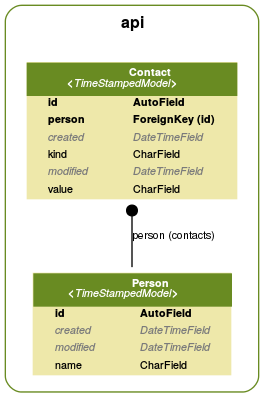
\includegraphics[width=.55\textwidth]{imagem/der.png}
  % Caption centralizada
  \captionsetup{justification=centering}
  \captionfont{\small{\textbf{\\Fonte: Autor}}}	
  \label{fig:der}
  \end{figure}
  
\section{Aplicação em Django}
\label{desenvolvimento-django}

  Falta algum texto

\section{Aplicação em Express.Js}
\label{escopo-projeto}

  Falta algum texto